%! Author = ιηмσяєѕєηтυм
%! Date = 4/2/23

\documentclass[conference]{IEEEtran}
\IEEEoverridecommandlockouts
% The preceding line is only needed to identify funding in the first footnote. If that is unneeded, please comment it out.
\usepackage{cite}
\usepackage{amsmath,amssymb,amsfonts}
\usepackage{algorithmic}
\usepackage{graphicx}
\usepackage{textcomp}
\usepackage{xcolor}
\usepackage{subfigure}
\usepackage{listings}

\def\BibTeX{{\rm B\kern-.05em{\sc i\kern-.025em b}\kern-.08em
T\kern-.1667em\lower.7ex\hbox{E}\kern-.125emX}}
\begin{document}

    \title{Design a 4-bit ALU\\
    {\footnotesize Group: \textit{4 CSE460 Lab Section 9}}
    }

    \author{\IEEEauthorblockN{ATHAR NOOR MOHAMMAD RAFEE}
    \IEEEauthorblockA{\textit{DEPT: CSE} \\
    \textit{ID: 20101396} \\
    Section: 9L \\
    noor.mohammad.rafee@g.bracu.ac.bd}
    \and

    \IEEEauthorblockN{A.S.M MAHABUB SIDDIQUI}
    \IEEEauthorblockA{\textit{DEPT: CSE} \\
    \textit{ID: 20301040} \\
    Section: 9L \\
    asm.mahabub.siddiqui@g.bracu.ac.bd}
    \and

    \IEEEauthorblockN{Ayon Das}
    \IEEEauthorblockA{\textit{DEPT: CSE)} \\
    \textit{ID: 20301099} \\
    Section: 9L \\
    ayon.das@g.bracu.ac.bd}
    \and

    \IEEEauthorblockN{MD. SAKIB}
    \IEEEauthorblockA{\textit{DEPT: CSE} \\
    \textit{ID: 20301180} \\
    Section: 9L \\
    md.sakib1@g.bracu.ac.bd}
    \and

    \IEEEauthorblockN{ MOHAMMED INZAM UL AZAM}
    \IEEEauthorblockA{\textit{DEPT: CSE} \\
    \textit{ID:20101144} \\
    Section: 09L \\
    mohammed.inzam.ul.azam@g.bracu.ac.bd}
    }

    \maketitle

    \begin{abstract}
        This project presents the design and implementation of a 4-bit Arithmetic Logic Unit (ALU).
        The ALU performs arithmetic and logical operations on two 4-bit inputs and produces a 4-bit output.
        The design is implemented using Verilog hardware description language and simulated using timing function.
        The ALU supports basic arithmetic operations such as addition and subtraction,
        as well as logical operations such as \textbf{ADD}, \textbf{NAND}, and \textbf{XNOR}
        as per requirements of the project.
        Overall, this project demonstrates the design and implementation of a simple but
        functional sequential ALU using Verilog HDL.
    \end{abstract}

    \begin{IEEEkeywords}
        ALU, Verilog, arithmetic, logic, simulation
    \end{IEEEkeywords}


    \section{Introduction}\label{sec:introduction}
    This report presents the design and implementation of a
4-bit ALU using Verilog HDL and Quartus II software.
The ALU was designed to perform various arithmetic
and logical operations such as \textbf{ADDITION}, \textbf{SUBTRACTION},
bitwise \textbf{AND}, bitwise \textbf{OR}, and bitwise \textbf{XOR}.
The design consists of various modules such as the Adder, Subtractor,
and logic gates which were generated based on the verilog code.
In this report, we provide a detailed description of the design and implementation process,
including the Verilog code for each module and the timing diagram for verification.
We also discuss the challenges encountered during the design process and how they were overcome.
Finally, we present the results of the hardware testing, demonstrating that
the ALU is capable of performing the desired operations accurately and efficiently.
The design of a 4-bit ALU is an essential component in digital circuit design,
and it is a fundamental building block in many larger circuits and VLSI design.


    \section{Finite State Machine Design and Implementation}\label{sec:FSM}
    Finite State Machine (FSM) is a model for designing sequential logic circuits,
where the circuit's behavior is determined by a finite number of states, inputs and outputs.
In this case, the FSM is designed to implement \textit{five} different operations,
namely RESET, XNOR, NAND, SUB, and ADD on two 4-bit inputs A and B.
The way we coded the Verilog code represents the implementation of the FSM,
which is designed to perform the above-mentioned arithmetic and logical operations on the given input values.
From an high level perspective, The \textbf{FSM} has Four states, which are encoded as 2-bit values, as follows:

\begin{figure}[H]
    \centerline{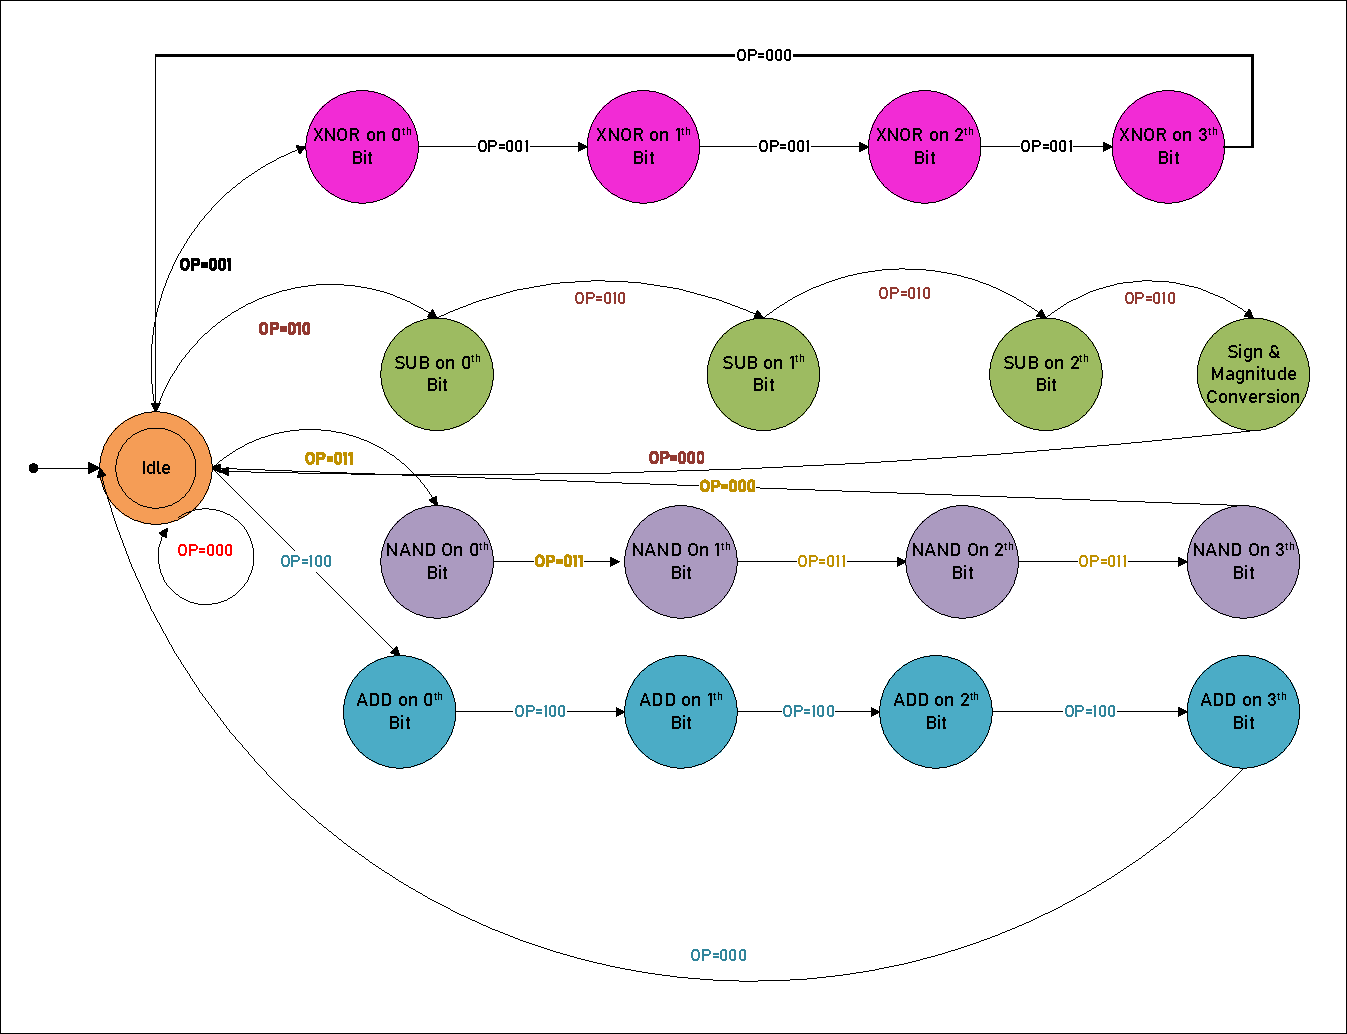
\includegraphics[height=6cm,width=6cm]{figures/FSM}}
    \caption{FSM Diagram}
    \label{fig:FSM}
\end{figure}

\begin{itemize}
    \item State 0 (\textit{2'b00}): In this state, the circuit performs the selected operation on the first bit of the input values and transitions to the next state.
    \item State 1 (\textit{2'b01}): In this state, the circuit performs the selected operation on the second bit of the input values and transitions to the next state.
    \item State 2 (\textit{2'b10}): In this state, the circuit performs the selected operation on the third bit of the input values and transitions to the next state.
    \item State 3 (\textit{2'b11}): In this state, the circuit performs the selected operation on the fourth and most significant bit of the input values and transitions back to the initial state.
\end{itemize}

Before transition, it also sets the values of \textit{zero} flag, \textit{sign} flag and \textit{carry} flag.


Things are checked and done slightly different based on the \textit{opcode}.
It can be observed from the above Fig \ref{fig:FSM} clearly.
The four different operations are implemented using a \textit{case} statement with \textit{opcode} as the selector.
Each operation \textit{case} statement contains the logic required to perform the operation on the given input values,
and update the output values of the circuit accordingly.
For example, for the \textbf{ADD} operation, the code first calculates the SUM of the LSBs of the input values,
adds the carry value to it (initially 0),
and assigns the SUM and the carry value to the output register \textbf{C}.
Then, it updates the \textit{zero} flag, which is set to 1 if the output is 0,
and transitions to the next state which is \textbf{IDLE} state that we can see from Figure \ref{fig:FSM}.
The outputs of the circuit include \textbf{C}, which stores the result of the operation,
\textit{carr}, which is the \textbf{carry} bit generated during addition or subtraction,
\textit{sign}, which is the sign bit of the output value, and zero, which is set to 1 if the output is \textit{0000}.
Overall, the FSM implementation allows the circuit to perform different arithmetic and logical
operations on the given input values, and update the output values based on the operation performed.


    \section{Verification}\label{sec:verification}
    After implementing the verilog code.
We used the timing function to verify the working of the code.
Below, we are attaching the screenshots from the timing diagram

\subsection{ADD Operation:}\label{subsec:add-operation}
Below figure \ref{fig:timing add} shows the \textbf{ADD} operation between two binary \textit{A = 1111 and B = 1111}
where the result is stored C sequentially in each clock cycles.
\begin{figure}[H]
    \begin{center}
        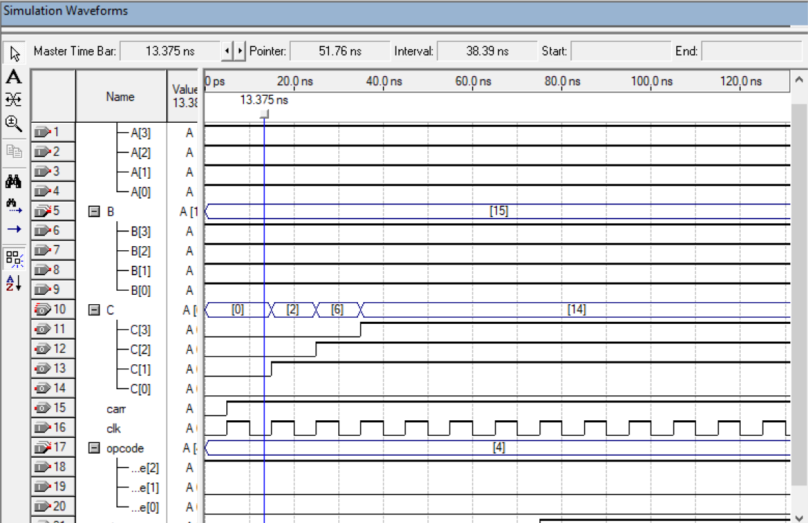
\includegraphics[width = 0.4\textwidth]{figures/add}
    \end{center}
    \caption{Timing Daigram for ADD Operation}
    \label{fig:timing add}
\end{figure}

\subsection{SUB Operation}\label{subsec:sub-operation}
Below figure \ref{fig:timing sub} shows the \textbf{SUB} operation between two binary \textit{A = 0111 and B = 0111}
\begin{figure}[H]
    \begin{center}
        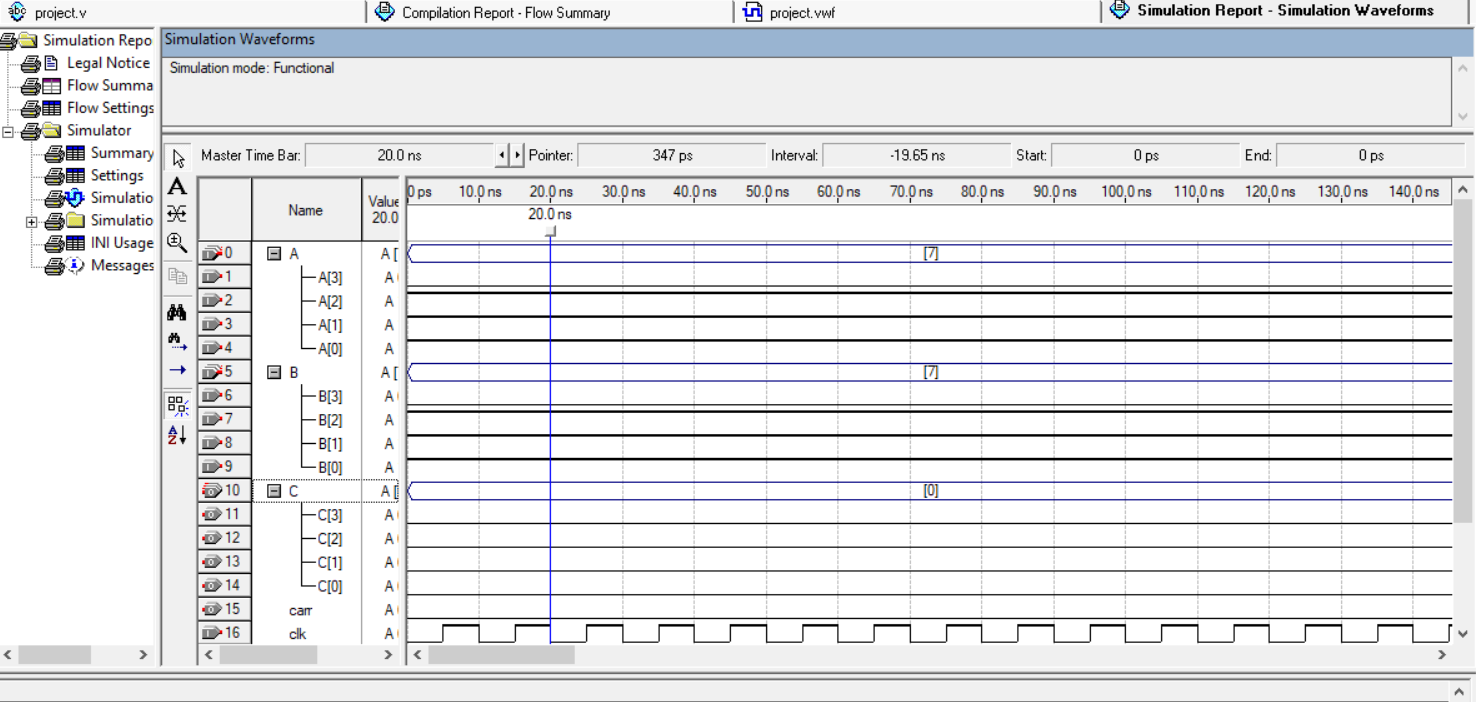
\includegraphics[width = 0.4\textwidth]{figures/sub_operation}
    \end{center}
    \caption{Timing Diagram for Sub Operation}
    \label{fig:timing sub}
\end{figure}

\textbf{NAND} and \textbf{XNOR} operation are pretty much straight forward.
All we had to do is put the equation in the verilog and then the
operation performed as expected.
Below timing diagram, those operations are attached.

\subsection{NAND Operation}\label{subsec:nand-operation}

\begin{figure}[H]
    \begin{center}
        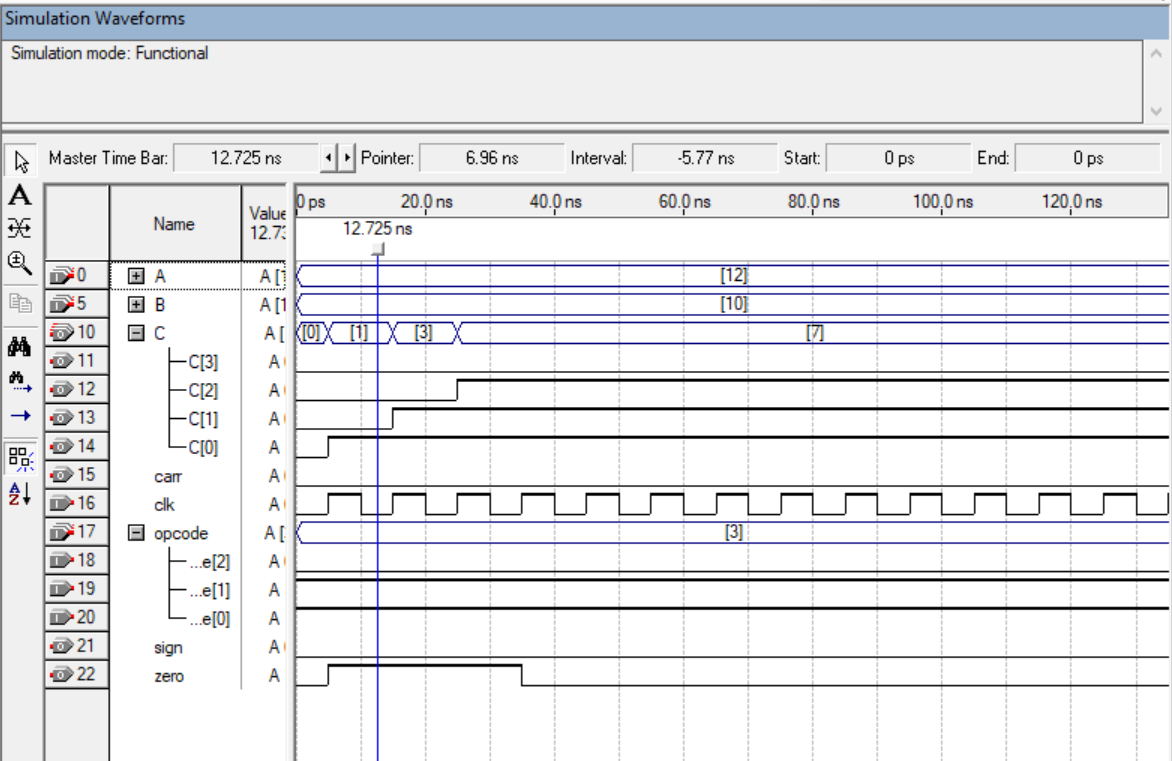
\includegraphics[width = 0.4\textwidth]{figures/nand}
    \end{center}
    \caption{Timing Daigram for NAND Operation}
    \label{fig:timing nand}
\end{figure}

\subsection{XNOR Operation}\label{subsec:xnor-operation}
\begin{figure}[H]
    \begin{center}
        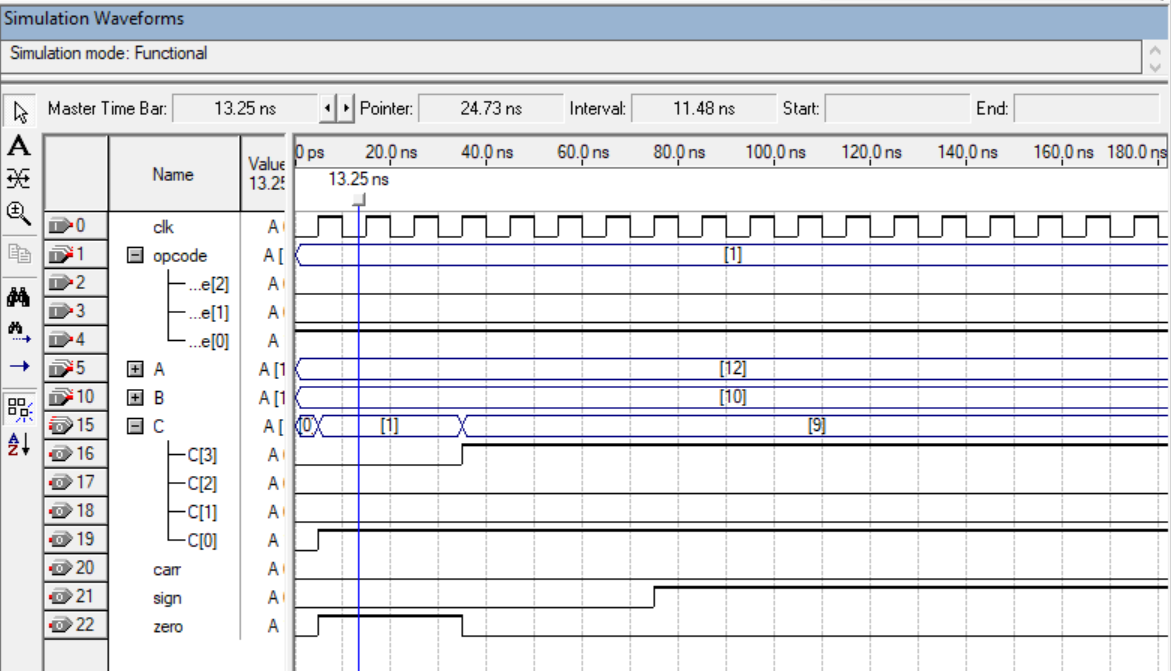
\includegraphics[width = 0.4\textwidth]{figures/xnor}
    \end{center}
    \caption{Timing Daigram for XNOR Operation}
    \label{fig:timing xnor}
\end{figure}

\subsection{Multiple Operation With Reset}\label{subsec:multiple-operation-with-reset}
The below attached Figure \ref{fig:multiple operation} shows multiple Operations with \textbf{SET} and \textbf{RESET} functionality.
At first the \textbf{SUB} operation is performed between binary number \textit{0111} and \textit{0111}.
After that, the \textbf{opcode} is changed to reset which is \textit{000} during time \textit{40ns} to \textit{50ns}.
Next, the \textbf{opcode} was changed to \textit{011} and performed \textbf{NANAD} operation during the next \textbf{4} clock cycles.
After that the mandatory \textbf{RESET} and then \textbf{ADD} operation for another 4 cycles.
\begin{figure}[H]
    \begin{center}
        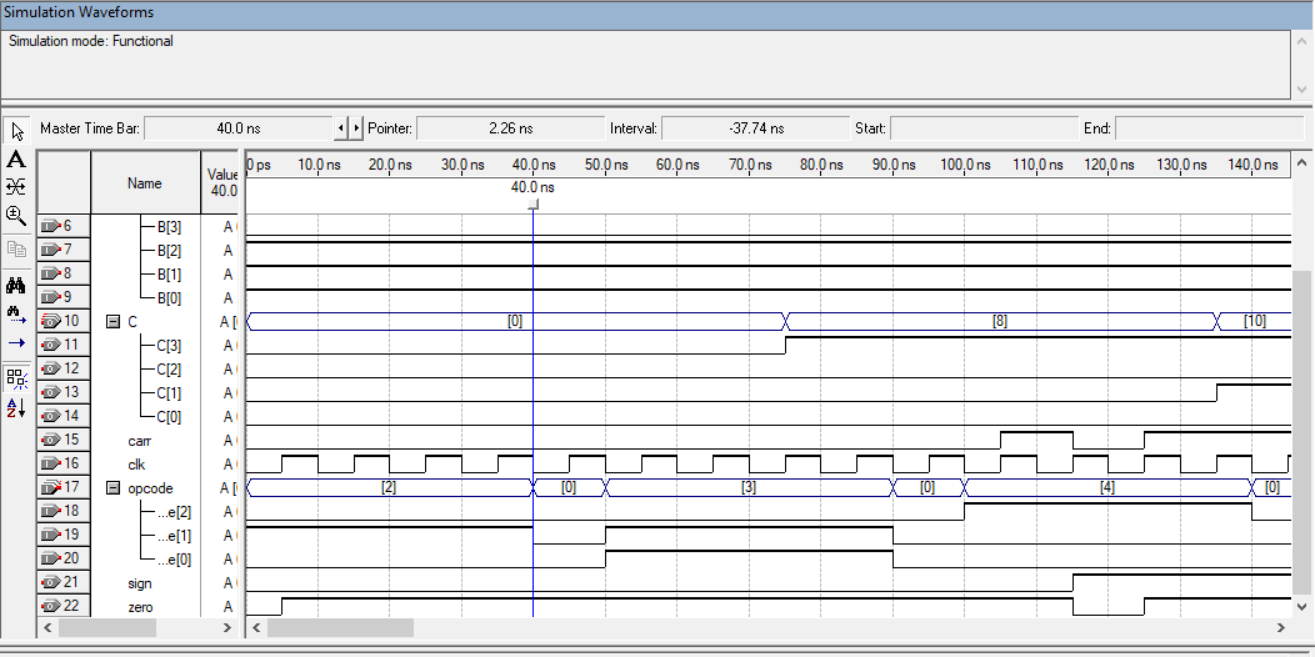
\includegraphics[width = 0.4\textwidth]{figures/three_operation_together_sub_nand_add_with_reset}
    \end{center}
    \caption{Timing Daigram with reset}
    \label{fig:multiple operation}
\end{figure}




    \section{Conclusion}\label{sec:conclusion}
    In conclusion, we have successfully designed and implemented a 4-bit ALU using finite state machines and \textit{Verilog HDL}.
We started by defining the project requirements and selecting the appropriate operations to be implemented.
Then, we designed the FSM with four states and carefully defined the transitions and outputs for each state.
We also implemented the FSM using Verilog HDL and simulated the design using timing diagram to verify its functionality.
The simulation results show that our design works correctly for all the selected operations and input combinations.
Finally, this project not only provided hands-on experience with Verilog HDL programming and digital circuit design, but also reinforced the
importance of a systematic approach to problem-solving and the importance of utilizing efficient design strategies.


    \appendix


    \section{Appendix}\label{sec:appendix}
    \lstdefinestyle{verilogStyle}{
    language=Verilog,
    basicstyle=\small\ttfamily,
    keywordstyle=\color{blue},
    commentstyle=\color{green},
    stringstyle=\color{purple},
    showstringspaces=false,
    breaklines=true,
    numbers=left,
    numberstyle=\tiny\color{gray},
    stepnumber=1,
    numbersep=4pt,
    frame=single,
    framerule=0pt,
    framesep=0pt,
    framexleftmargin=5pt,
    xleftmargin=10pt,
    tabsize=4,
    captionpos=b,
    floatplacement=tbhp
}

\subsection{Verilog HDL Code}\label{subsec:verilog-hdl-code}
\begin{lstlisting}[style=verilogStyle, caption={Verilog code for 4-bit ALU},label={lst:lstlisting}]
module project(input clk, input [3:0] A, input [3:0] B,
 input [2:0] opcode, output reg [3:0] C,
  output reg carr, output reg sign, output reg zero);
// Will be using state to indicate state of the machine.
reg [1:0] state = 0;
always @ (posedge clk) begin
    case (state)
        2'b00: begin
            case (opcode)
                3'b000: begin
                    C <= 4'b0000; //RESET operation
                    carr <= 1'b0;
                    sign <= 1'b0;
                    zero <= 1'b1;
                end
                3'b001: begin //XNOR operation on LSBs
                    C[0] <= ~(A[0] ^ B[0]);
                    zero <= C[0] == 1'b0;
                end
                3'b010: begin //SUB operation on LSBs
                    {carr, C[0]} <= B[0] - A[0];
                    zero <= C[0] == 1'b0;
               end
                3'b011: begin //NAND operation on LSBs
                    C[0] <= ~(A[0] & B[0]);
                    zero <= C[0] == 1'b0;
                end
                3'b100: begin //ADD operation on LSBs
                    {carr, C[0]} <= A[0] + B[0];
                    zero <= C[0] == 1'b0;
                end


            endcase
            state <= 2'b01;
        end
        2'b01: begin
            case (opcode)
                3'b001: begin //XNOR operation on next bit
                    C[1] <= ~(A[1] ^ B[1]);
                    zero <= zero & (C[1] == 1'b0);
                end
                3'b010: begin //SUB operation on next bit
                    {carr, C[1]} <= B[1] - A[1] - carr;
                    zero <= zero & (C[1] == 1'b0);
                end
                3'b011: begin //NAND operation on next bit
                    C[1] <= ~(A[1] & B[1]);
                    zero <= zero & (C[1] == 1'b0);
                end
                3'b100: begin //ADD operation on next bit
                    {carr, C[1]} <= A[1] + B[1] + carr;
                    zero <= zero & (C[1] == 1'b0);
                end


            endcase
            state <= 2'b10;
        end
        2'b10: begin
            case (opcode)
                3'b001: begin //XNOR operation on next bit
                    C[2] <= ~(A[2] ^ B[2]);
                    zero <= zero & (C[2] == 1'b0);
                end
                3'b010: begin //SUB operation on next bit
                    {carr, C[2]} <= B[2] - A[2] - carr;
                    zero <= zero & (C[2] == 1'b0);
                end
                3'b011: begin //NAND operation on next bit
                    C[2] <= ~(A[2] & B[2]);
                    zero <= zero & (C[2] == 1'b0);
                end
                3'b100: begin //ADD operation on next bit
                    {carr, C[2]} <= A[2] + B[2] + carr;
                    zero <= zero & (C[2] == 1'b0);
                end

            endcase
            state <= 2'b11;
        end
        2'b11: begin
            case (opcode)
                3'b001: begin //XNOR operation on MSBs
                    C[3] <= ~(A[3] ^ B[3]);
                    sign <= C[3];
                    zero <= C == 4'b0000;
                end
                3'b010: begin //SUB operation on MSBs
                 {carr, C[3]} <= B[3] - A[3] - carr;
                 sign <= C[3];
                 zero <= C == 4'b0000;
                   if (B[3] < A[3]) begin //if result is negative, take two's complement of result
                       C <= ~C + 4'b0001;
                       sign <= C[3];
                   end
                end
                3'b011: begin //NAND operation on MSBs
                                    C[3] <= ~(A[3] & B[3]);
                    sign <= C[3];
                    zero <= C == 4'b0000;
                end
                3'b100: begin //ADD operation on MSBs
                    {carr, C[3]} <= A[3] + B[3] + carr;
                    sign <= C[3];
                    zero <= C == 4'b0000;
                end

            endcase
            state <= 2'b00;
        end
    endcase
end
endmodule
\end{lstlisting}


\end{document}
